\documentclass[12pt]{book}
\usepackage[utf8]{inputenc}
\usepackage{lmodern}
\usepackage{amsmath,amssymb,amsthm}
\usepackage{hyperref}
\usepackage{graphicx}
\usepackage{tikz}
\usepackage{minted}
\usepackage{enumitem}
\setlist{noitemsep}

\usepackage{tcolorbox}
\tcbuselibrary{listings,minted,skins}

\newtcblisting{pythoncode}{
  listing engine=minted,
  colback=blue!5!white,
  colframe=blue!75!black,
  listing only,
  minted language=python,
  minted options={fontsize=\small,breaklines,autogobble,linenos,numbersep=3mm},
  left=5mm,
  enhanced,
  title=Python Implementation,
  arc=0.3mm,
  boxrule=0.8pt
}


\title{A Mathematical Introduction to Large Language Models}
\author{Author Name}
\date{\today}

\begin{document}

\maketitle

\tableofcontents

\part{Foundations}
% PROMPT: Introduce the overall scope and purpose of the book

\chapter{Introduction to Large Language Models}
% PROMPT: Provide historical milestones of LLM development
\section{Historical Development of LLMs}
\label{sec:historical}
\noindent
Language modeling has been a central challenge in Natural Language Processing (NLP) for decades. Researchers have continually sought methods to better predict or generate text based on observed patterns in language data. In this section, we examine the progression of language models, starting from the simplicity of n-gram models and moving toward the transformative impact of modern large-scale Transformer-based architectures.


\subsection{Early Language Models (n-grams)}
\label{sec:early_n_grams}
% PROMPT: Explain what n-grams are and how they paved the way for more advanced language models

\noindent
An \textbf{n-gram} model is one of the earliest approaches to language modeling. It is based on the \emph{Markov assumption}, which simplifies the probability of the next word in a sequence by conditioning only on a fixed number of preceding words. Specifically, an n-gram model approximates the probability of a word $w_t$ given its entire history $\{w_1, w_2, \ldots, w_{t-1}\}$ by considering only the previous $n-1$ words:

\[
P(w_t \mid w_1, w_2, \ldots, w_{t-1}) \approx P(w_t \mid w_{t-(n-1)}, \ldots, w_{t-1}).
\]

\noindent
Here, $n$ indicates how many words (or tokens) we look back in the sequence. The simplest examples include:
\begin{itemize}
    \item \textbf{Unigram model ($n = 1$):}
    \[
    P(w_t) \approx \text{frequency of } w_t,
    \]
    which ignores any context and simply assigns probabilities based on overall word frequencies.

    \item \textbf{Bigram model ($n = 2$):}
    \[
    P(w_t \mid w_{t-1}) \approx \frac{\text{count}(w_{t-1}, w_t)}{\text{count}(w_{t-1})},
    \]
    where the probability of $w_t$ depends only on the immediately preceding word $w_{t-1}$.

    \item \textbf{Trigram model ($n = 3$):}
    \[
    P(w_t \mid w_{t-1}, w_{t-2}) \approx \frac{\text{count}(w_{t-2}, w_{t-1}, w_t)}{\text{count}(w_{t-2}, w_{t-1})}.
    \]
\end{itemize}

\noindent
While these models offer a simple yet effective approach for small-scale language tasks, they suffer from several drawbacks:
\begin{enumerate}
    \item \textbf{Data Sparsity.} As $n$ increases, the number of possible n-grams grows exponentially, making it extremely difficult to obtain reliable probability estimates from finite data. Many n-grams may never appear in the training corpus, leading to zero probabilities.
    \item \textbf{Limited Context Window.} Even with higher-order n-grams, the model can only capture a short context window. This limitation means the model struggles to handle long-range dependencies or global context in a sentence or document.
    \item \textbf{Smoothing Techniques.} To address sparsity, methods such as \emph{Laplace smoothing}, \emph{Kneser-Ney smoothing}, and others are commonly employed. However, these strategies merely mitigate the issue and do not fundamentally solve the limitations of the n-gram framework.
\end{enumerate}

\noindent
Despite their simplicity and shortcomings, n-gram models laid an important foundation for statistical language modeling. They introduced fundamental ideas such as using frequency counts and conditional probabilities for word prediction. These core principles influenced the development of more sophisticated neural language models that emerged with the advent of deeper architectures, larger corpora, and more powerful computational resources.

\subsection{Transition to Neural Language Models}
\label{sec:transition_nn_models}
% PROMPT: Discuss the shift from statistical approaches to neural network-based language models

\noindent
While n-gram models offered a foundational statistical approach to language modeling, they were increasingly limited by their inability to capture long-range dependencies. This shortcoming, in tandem with growing computational capabilities, paved the way for \textbf{neural language models}. The foundational work on backpropagation by \emph{Rumelhart et al.}~\cite{rumelhart1986learning} and early experiments with simple recurrent networks by \emph{Elman}~\cite{elman1990finding} laid the groundwork for neural approaches to sequence modeling.

\begin{itemize}
    \item \textbf{The Introduction of Distributed Representations.}
    Pioneering work by \emph{Bengio et al.}~\cite{bengio2003neural} introduced the concept of learned word embeddings, replacing one-hot word vectors with dense, low-dimensional representations. This shift helped alleviate data sparsity and allowed models to generalize better to unseen n-grams by placing related words closer together in the embedding space.

    \item \textbf{The Rise of Recurrent Neural Networks (RNNs).}
    RNN-based architectures~\cite{graves2013generating} quickly became a popular choice for sequence modeling. By maintaining a hidden state that is updated at each time step, RNNs can theoretically encode information from all previous tokens in a sequence. 
    \begin{itemize}
        \item \textit{Vanilla RNNs} often faced vanishing or exploding gradients when handling long sequences~\cite{pascanu2013difficulty}, leading to difficulties in capturing context over longer spans of text.
        \item \textit{Long Short-Term Memory (LSTM)}~\cite{hochreiter1997long} networks and \textit{Gated Recurrent Units (GRUs)}~\cite{cho2014learning} introduced gating mechanisms to mitigate these gradient issues, enabling better information flow across many time steps.
    \end{itemize}
    Despite their improvements over n-gram models, RNN-based architectures were still computationally intensive, often needing sequential processing for each token.

    \item \textbf{Introduction of Word2Vec and Glove.}
    Around the same time, \texttt{Word2Vec} and \texttt{Glove} emerged as popular methods for learning distributed word representations outside of a full neural language model framework. These methods optimized simpler objectives (e.g., skip-gram, continuous bag-of-words, or global co-occurrence matrices) to produce embeddings that captured semantic and syntactic regularities.

    \item \textbf{Limitations and the Search for Parallelism.}
    Although RNNs and LSTMs represented a breakthrough in language modeling, they remained sequential in nature—each token's representation depended on the previous token's output. This sequential dependency limited parallelization and made training on extremely large corpora slow and costly. Researchers began to explore alternative architectures that could better exploit GPU parallelism and handle longer contexts without exponential growth in training time.
\end{itemize}

\noindent
In short, the transition to neural language models marked a pivotal moment in NLP, broadening the scope of what language models could achieve. By leveraging distributed representations and more flexible architectures, these models began to surpass traditional statistical methods on a range of language tasks. However, it would take the subsequent step of discarding recurrence altogether and introducing the \textbf{attention mechanism} before truly massive-scale language models, often referred to as \textit{Large Language Models}, could flourish.

\subsection{The Emergence of Transformers and LLMs}
\label{sec:transformers_llms}
% PROMPT: Highlight how the Transformer architecture revolutionized NLP and led to massive LLMs

\noindent
Building on the foundations laid by RNN-based approaches~\cite{hochreiter1997long}, the \textbf{Transformer} architecture, introduced by \emph{Vaswani et al.}~\cite{vaswani2017attention} in 2017, marked a paradigm shift in Natural Language Processing (NLP). Instead of relying on recurrent connections (or convolutions) to process sequences, Transformers use a fully \emph{attention-based} mechanism to model complex dependencies in parallel. This design not only alleviated many of the bottlenecks found in RNNs but also enabled significant performance improvements across a broad spectrum of NLP tasks.

\begin{itemize}
    \item \textbf{Key Innovation: Self-Attention.} 
    The Transformer's core operation, called \textit{self-attention}, allows the model to weigh the importance of different parts of a sequence to each other \emph{in parallel}, without processing tokens one at a time. This is especially advantageous for capturing long-range dependencies since each token can "attend to" any other token directly. Moreover, it opens the door for massively parallel computations on modern GPUs or TPUs.

    \item \textbf{Positional Encoding and Multi-Head Attention.}
    Because Transformers discard recurrence, they need a method to encode the order of tokens in a sequence. \emph{Positional encoding} injects information about token positions through either sinusoidal or learned embeddings. The model also employs \textit{multi-head attention}, which processes attention in multiple parallel subspaces, allowing it to capture diverse relationships within the input.

    \item \textbf{Scalability and Performance.}
    With attention-based operations, Transformers proved substantially more scalable than RNNs. Training could be distributed over large GPU clusters, and the architecture could handle \emph{very} long context windows effectively. This scalability was quickly exploited by researchers and industry practitioners~\cite{brown2020language}, who trained Transformers on massive text corpora, producing what are now commonly called \textbf{Large Language Models (LLMs)}.

    \item \textbf{Examples of LLMs: BERT, GPT, and Beyond.}
    Since the debut of the Transformer, several influential LLMs have emerged:
    \begin{itemize}
        \item \textit{BERT (Bidirectional Encoder Representations from Transformers)}~\cite{devlin2018bert} demonstrated the power of masked language modeling for capturing bidirectional context, achieving state-of-the-art results on numerous NLP benchmarks.
        
        \item \textit{GPT (Generative Pretrained Transformer)} series~\cite{radford2018improving,radford2019language} focused on unidirectional (left-to-right) language modeling, enabling impressive generative capabilities and pioneering few-shot and zero-shot learning approaches when scaled up.
        
        \item Subsequent models like \textit{T5}~\cite{raffel2020exploring}, \textit{XLNet}~\cite{yang2019xlnet}, and \textit{RoBERTa}~\cite{liu2019roberta} introduced new training objectives, larger parameter counts, and improved performances on benchmarks from question answering to machine translation.
    \end{itemize}

    \item \textbf{Impact on the Field.}
    The rise of LLMs profoundly changed NLP research and practice. Tasks that once required domain-specific feature engineering began to be addressed by general-purpose, pre-trained Transformers fine-tuned with minimal additional data. Moreover, LLMs have revealed surprising emergent properties in natural language understanding, reasoning, and even creative text generation—motivating research into interpretability, bias mitigation, and ethical deployment.

\end{itemize}

\noindent
In essence, the Transformer and its descendants ushered in a new age of NLP, where models capable of \emph{scaling} to billions (and even trillions) of parameters dominate the landscape. As we explore these architectures further in subsequent chapters, we will highlight the key mathematical concepts and training strategies that have enabled LLMs to become a cornerstone of modern AI applications.

% PROMPT: Expand on the evolution from n-gram models to modern Transformers


% PROMPT: Compare small language models to large language models in more detail
\section{What Makes LLMs Different?}\index{LLM!differences}\index{language models!large vs small}
\label{sec:llms_difference}
% PROMPT: Compare small language models to large language models in more detail

\noindent
While traditional language models\index{language models!traditional}—be they n-gram\index{n-gram models} or smaller neural architectures\index{neural architectures!small}—have contributed substantially to various NLP tasks\index{NLP tasks}, \textbf{Large Language Models (LLMs)}\index{LLM|see {Large Language Model}}\index{Large Language Model} stand apart in terms of scale\index{scale}, performance\index{performance}, and versatility\index{versatility}. This section explores some of the key attributes that differentiate LLMs from their predecessors\index{model predecessors}.

\begin{itemize}
    \item \textbf{Scale and Parameter Count.}\index{scale!parameters}\index{parameter count}
    One of the most defining characteristics of an LLM is its sheer size\index{model size}. These models can contain billions\index{parameters!billions} (or even trillions\index{parameters!trillions}) of parameters, far surpassing the capacity of earlier architectures\index{model capacity}. Such expansive parameter spaces\index{parameter space} allow LLMs to store rich linguistic\index{linguistic information} and factual information\index{factual information}, leading to improved performance on diverse tasks\index{task diversity}, from text classification\index{text classification} to creative text generation\index{text generation!creative}. However, training\index{training!computational requirements} and serving\index{model serving} these enormous models come with steep computational\index{computational requirements} and memory requirements\index{memory requirements}, motivating significant research into distributed systems\index{distributed systems} and model parallelism\index{model parallelism}.

    \item \textbf{Data Requirements and Training Pipelines.}\index{data requirements}\index{training pipelines}
    LLMs are typically pre-trained\index{pre-training} on massive text corpora\index{text corpora} scraped from the web\index{web scraping}, encompassing a wide variety of styles\index{text styles}, domains\index{domains}, and languages\index{languages}. This \emph{pre-training phase}\index{pre-training phase} enables the model to learn general-purpose representations\index{representations!general-purpose} of language before being adapted to specific tasks. The construction of such large-scale datasets\index{datasets!large-scale} often involves:
    \begin{itemize}
        \item Web crawling\index{web crawling} and cleaning\index{data cleaning} to remove noise\index{noise removal} and inappropriate content\index{content filtering}.
        \item Tokenization\index{tokenization} or text normalization\index{text normalization} steps to convert raw text into manageable tokens\index{tokens}.
        \item Automated filtering\index{automated filtering} to reduce duplication\index{duplication reduction} and protect privacy\index{privacy protection} where possible.
    \end{itemize}
    This pre-training pipeline\index{pre-training pipeline}, coupled with advanced optimization methods\index{optimization methods}, allows LLMs to \emph{self-supervise}\index{self-supervision} on unlabeled text\index{unlabeled text}, capturing vast contextual\index{contextual knowledge} and semantic knowledge\index{semantic knowledge}.

    \item \textbf{Impact on Natural Language Tasks and Applications.}\index{natural language tasks}\index{applications}
    Once pre-trained, LLMs can be fine-tuned\index{fine-tuning} or prompted\index{prompting} to perform exceptionally well on a broad array of downstream tasks\index{downstream tasks}:
    \begin{itemize}[noitemsep]
        \item \textit{Reading Comprehension \& Question Answering:}\index{reading comprehension}\index{question answering} LLMs can interpret context passages\index{context interpretation} and provide answers with a depth that surpasses smaller models.
        \item \textit{Text Generation \& Summarization:}\index{text generation}\index{summarization} By leveraging expansive learned knowledge\index{learned knowledge}, LLMs produce cohesive summaries\index{summaries} and human-like text\index{human-like text} in various domains.
        \item \textit{Zero-Shot \& Few-Shot Learning:}\index{zero-shot learning}\index{few-shot learning} Owing to their large pre-training corpus, LLMs can tackle new tasks with minimal or even no explicit examples, demonstrating emergent generalization skills\index{generalization skills}.
        \item \textit{Creative Tasks:}\index{creative tasks} LLMs' generative prowess\index{generative capabilities} allows them to assist in writing prose\index{prose writing}, poetry\index{poetry}, or even computer code\index{code generation}, showcasing impressive degrees of fluency\index{fluency} and coherence\index{coherence}.
    \end{itemize}
    This versatility increasingly positions LLMs as a \emph{universal backbone}\index{universal backbone} for NLP applications\index{NLP applications}, transforming how researchers and practitioners approach natural language tasks.

    \item \textbf{Challenges and Considerations.}\index{challenges}\index{considerations}
    With great power comes great responsibility. LLMs raise pressing concerns around:
    \begin{enumerate}
        \item \textbf{Ethical and Bias Issues:}\index{ethical issues}\index{bias issues} LLMs can inadvertently learn and propagate societal biases\index{societal biases} present in their training data, creating potential harm\index{potential harm} in real-world applications\index{real-world applications}.
        \item \textbf{Computational Costs:}\index{computational costs} Training and deploying LLMs require considerable computational resources\index{computational resources}, making them less accessible\index{accessibility} to smaller research groups\index{research groups} and increasing the environmental footprint\index{environmental footprint}.
        \item \textbf{Interpretability and Control:}\index{interpretability}\index{control} As models grow more complex\index{model complexity}, understanding their decision-making processes\index{decision-making} becomes challenging, raising questions about transparency\index{transparency} and reliability\index{reliability}.
    \end{enumerate}
    These challenges underscore the necessity for ongoing research in techniques like parameter-efficient fine-tuning\index{parameter-efficient fine-tuning}, model compression\index{model compression}, bias detection\index{bias detection}, and interpretability frameworks\index{interpretability frameworks}.

\end{itemize}

\noindent
In sum, LLMs differentiate themselves through their capacity to learn universal linguistic representations from massive data, adapt quickly to new tasks, and generate highly coherent text. Their ever-growing size, however, entails significant engineering, ethical, and societal considerations, making it crucial for future work to balance innovation with responsible deployment. 


% PROMPT: Provide a roadmap of the book’s structure
\section{Organization of the Book}
\label{sec:book_organization}
% PROMPT: Provide a roadmap of the book’s structure

\noindent
The purpose of this book is to provide a comprehensive overview of Large Language Models (LLMs) and the mathematics that underpins them, from foundational concepts to advanced techniques. To help you navigate the material, the book is divided into five main parts, each focusing on a key aspect of LLMs:

\begin{itemize}
    \item \textbf{Part I: Foundations.} 
    This section covers the essential mathematical background—including linear algebra, calculus, probability, and basic machine learning concepts—necessary to understand the more complex ideas presented later in the book.

    \item \textbf{Part II: Transformer Architecture and Attention.} 
    Here, we delve into the core building blocks of modern LLMs. We unpack the attention mechanism, explore how it is scaled up through multi-head attention, and examine the complete Transformer encoder-decoder structure that revolutionized NLP.

    \item \textbf{Part III: Training Large Language Models.}
    This section focuses on the training objectives for language modeling, large-scale optimization techniques, and practical considerations for scaling up to billions of parameters. We also discuss hyperparameter tuning strategies and the empirical scaling laws that guide model growth.

    \item \textbf{Part IV: Advanced Topics and Future Directions.}
    Beyond the essentials, we look at fine-tuning methods, prompt engineering, interpretability, and bias concerns. We also explore how LLMs can be distilled or compressed for efficient deployment, and discuss the latest frontiers like multimodal models and reinforcement learning integrations.

    \item \textbf{Part V: Conclusion and Resources.}
    The book concludes with a summary of the key mathematical concepts and practical takeaways, along with pointers to additional resources such as research papers, code libraries, and online courses. 

\end{itemize}

\noindent
Throughout each part, you will find both theoretical explanations and practical implementations. Where possible, we provide step-by-step derivations of key formulas, code snippets, and hands-on exercises to reinforce learning. By the end of the book, our aim is for you to have both a solid mathematical grounding in LLMs and the practical know-how to experiment with—and even innovate upon—this rapidly evolving class of models.



\chapter{Essential Mathematics}
% PROMPT: Summarize key linear algebra concepts needed for LLMs
\section{Linear Algebra}
\begin{itemize}
    \item Vector spaces, norms, and inner products
    \item Matrices: multiplication, inversion, eigenvalues/eigenvectors
    \item Decompositions: SVD and PCA in the context of dimensionality reduction
\end{itemize}

% PROMPT: Connect calculus topics to neural network training
\section{Calculus Refresher}
\begin{itemize}
    \item Derivatives and gradients
    \item Chain rule and partial derivatives
    \item Vector calculus essentials (Jacobian, Hessian)
\end{itemize}

% PROMPT: Provide additional probability examples relevant to NLP
\section{Probability and Statistics}
\begin{itemize}
    \item Basic probability distributions (Gaussian, Bernoulli, etc.)
    \item Expected values and variance
    \item Entropy and cross-entropy
\end{itemize}

% PROMPT: Include hands-on matrix factorization examples
\section{Exercises and Examples}
\begin{itemize}
    \item Hands-on linear algebra manipulations (e.g., matrix factorization)
    \item Simple probability calculations relevant to language modeling
\end{itemize}


\chapter{Machine Learning Fundamentals}
% PROMPT: Provide code examples of popular loss functions

\section{Review of Supervised and Unsupervised Learning}
\label{sec:review_of_supervised_and_unsupervised_learning}

Before diving into the specifics of Large Language Models, it's helpful to review the fundamental concepts of supervised and unsupervised learning, as these form the foundation for understanding more complex machine learning systems.

\subsection{Supervised Learning}

Supervised learning is a paradigm where models learn from labeled data pairs $(x, y)$, where $x$ represents the input features and $y$ represents the target output. The goal is to learn a function $f$ that maps inputs to outputs: $f: X \rightarrow Y$.

\subsubsection{Key Characteristics}
\begin{itemize}[noitemsep]
    \item Requires labeled training data
    \item Has clear evaluation metrics
    \item Learns explicit input-output mappings
\end{itemize}

\subsubsection{Common Applications}
\begin{itemize}[noitemsep]
    \item Classification (e.g., spam detection, image recognition)
    \item Regression (e.g., price prediction, temperature forecasting)
    \item Sequence labeling (e.g., part-of-speech tagging)
\end{itemize}

\subsubsection{Loss Functions}
In supervised learning, loss functions quantify how well our model's predictions match the true values. Different tasks require different loss functions:

\paragraph{Mean Squared Error (MSE)}
Commonly used for regression tasks, MSE measures the average squared difference between predictions and true values:

\[ MSE = \frac{1}{n}\sum_{i=1}^n (y_i - \hat{y}_i)^2 \]

Figure \ref{fig:mse_implementation} shows a simple NumPy implementation of MSE loss.

\begin{figure}[h]
\begin{pythoncode}
import numpy as np

def mse_loss(y_true, y_pred):
    return np.mean((y_true - y_pred) ** 2)

# Example usage
y_true = np.array([1.0, 2.0, 3.0])
y_pred = np.array([1.1, 2.2, 2.8])
loss = mse_loss(y_true, y_pred)  # Output: 0.05
\end{pythoncode}
\caption{Implementation of Mean Squared Error loss function}
\label{fig:mse_implementation}
\end{figure}

\paragraph{Cross-Entropy Loss}
Used primarily for classification tasks, cross-entropy loss measures the difference between predicted probability distributions and true labels:

\[ H(y, \hat{y}) = -\sum_{i=1}^n y_i \log(\hat{y}_i) \]

The implementation of cross-entropy loss with numerical stability considerations is shown in Figure \ref{fig:cross_entropy_implementation}.

\begin{figure}[h]
\begin{pythoncode}
def cross_entropy_loss(y_true, y_pred):
    # Add small epsilon to avoid log(0)
    epsilon = 1e-15
    y_pred = np.clip(y_pred, epsilon, 1 - epsilon)
    return -np.sum(y_true * np.log(y_pred))

# Example for binary classification
y_true = np.array([1, 0, 1])
y_pred = np.array([0.9, 0.1, 0.8])
loss = cross_entropy_loss(y_true, y_pred)
\end{pythoncode}
\caption{Implementation of Cross-Entropy loss function with numerical stability}
\label{fig:cross_entropy_implementation}
\end{figure}

\subsubsection{Optimization Algorithms}
The process of minimizing loss functions typically involves gradient descent and its variants.

\paragraph{Stochastic Gradient Descent (SGD)}
Basic SGD updates parameters using the gradient of the loss with respect to each parameter:

\[ \theta_{t+1} = \theta_t - \eta \nabla_\theta J(\theta) \]

A basic implementation of SGD is shown in Figure \ref{fig:sgd_implementation}.

\begin{figure}[h]
\begin{pythoncode}
def sgd_update(params, grads, learning_rate=0.01):
    return params - learning_rate * grads

# Example usage
weights = np.array([0.5, -0.2, 0.1])
gradients = np.array([0.1, -0.05, 0.02])
weights = sgd_update(weights, gradients)
\end{pythoncode}
\caption{Implementation of basic Stochastic Gradient Descent}
\label{fig:sgd_implementation}
\end{figure}

\paragraph{SGD with Momentum}
Momentum helps accelerate SGD by accumulating a velocity vector in directions of persistent reduction in the objective. Figure \ref{fig:momentum_implementation} demonstrates the implementation of SGD with momentum.

\begin{figure}[h]
\begin{pythoncode}
def sgd_momentum_update(params, velocity, grads, 
                       learning_rate=0.01, momentum=0.9):
    velocity = momentum * velocity - learning_rate * grads
    return params + velocity, velocity

# Example usage
weights = np.array([0.5, -0.2, 0.1])
velocity = np.zeros_like(weights)
gradients = np.array([0.1, -0.05, 0.02])
weights, velocity = sgd_momentum_update(weights, velocity, gradients)
\end{pythoncode}
\caption{Implementation of SGD with Momentum}
\label{fig:momentum_implementation}
\end{figure}

\paragraph{Adam Optimizer}
Adam combines ideas from momentum and RMSprop, maintaining per-parameter learning rates. The implementation with bias correction is shown in Figure \ref{fig:adam_implementation}.

\begin{figure}[h]
\begin{pythoncode}
def adam_update(params, m, v, grads, t, 
                learning_rate=0.001, beta1=0.9, beta2=0.999):
    epsilon = 1e-8
    
    # Update biased first moment estimate
    m = beta1 * m + (1 - beta1) * grads
    # Update biased second moment estimate
    v = beta2 * v + (1 - beta2) * grads**2
    
    # Bias correction
    m_hat = m / (1 - beta1**t)
    v_hat = v / (1 - beta2**t)
    
    # Update parameters
    params = params - learning_rate * m_hat / (np.sqrt(v_hat) + epsilon)
    return params, m, v

# Example usage
weights = np.array([0.5, -0.2, 0.1])
m = np.zeros_like(weights)
v = np.zeros_like(weights)
gradients = np.array([0.1, -0.05, 0.02])
t = 1  # timestep
weights, m, v = adam_update(weights, m, v, gradients, t)
\end{pythoncode}
\caption{Implementation of Adam optimizer with bias correction}
\label{fig:adam_implementation}
\end{figure}

\subsection{Practical Considerations}

When implementing these optimization algorithms, several factors should be considered:

\begin{itemize}[noitemsep]
    \item Learning rate selection is crucial and often requires tuning
    \item Batch size affects both training stability and computational efficiency
    \item Initialization of parameters can significantly impact convergence
    \item Regularization techniques help prevent overfitting
\end{itemize}

\subsection{Unsupervised Learning}

Unsupervised learning involves finding patterns or structure in unlabeled data. Unlike supervised learning, there are no explicit target outputs to learn from.

\subsubsection{Key Characteristics}
\begin{itemize}[noitemsep]
    \item Works with unlabeled data
    \item Focuses on finding patterns and structure
    \item Often more exploratory in nature
\end{itemize}

\subsubsection{Common Applications}
\begin{itemize}[noitemsep]
    \item Clustering (e.g., customer segmentation)
    \item Dimensionality reduction (e.g., PCA, t-SNE)
    \item Anomaly detection
\end{itemize}

\subsection{The Bridge to Language Models}

Understanding these fundamental learning paradigms is crucial for grasping how Large Language Models work, as they incorporate aspects of both:

\begin{itemize}[noitemsep]
    \item Like supervised learning, LLMs learn patterns from input-output pairs during pre-training (e.g., predicting the next word)
    \item Like unsupervised learning, they discover latent patterns and structures in language without explicit labeling
    \item They introduce new concepts like self-supervision, where the supervision signal is automatically derived from the input data itself
\end{itemize}

\subsection{Key Differences in Scale and Approach}

Traditional supervised and unsupervised learning typically operate on:
\begin{itemize}[noitemsep]
    \item Smaller, carefully curated datasets
    \item Well-defined problem spaces
    \item Specific tasks with clear evaluation metrics
\end{itemize}

In contrast, modern LLMs:
\begin{itemize}[noitemsep]
    \item Use massive datasets (billions of tokens)
    \item Learn general-purpose representations
    \item Can adapt to multiple tasks without task-specific training
\end{itemize}

This foundation in classical machine learning concepts helps us better understand both the innovations and limitations of modern language models, which we'll explore in subsequent chapters. 
% \begin{itemize}
%     \item Loss functions (MSE, cross-entropy)
%     \item Gradient descent and its variants (SGD, momentum, Adam)
% \end{itemize}

% PROMPT: Showcase a minimal neural network from scratch
% \section{Neural Networks 101}
\section{Neural Networks 101}\index{neural networks}\index{neural networks!basics}
\label{sec:neural_networks_101}
% PROMPT: Showcase a minimal neural network from scratch

\subsection{Perceptrons and Multi-Layer Perceptrons (MLPs)}\index{perceptron}\index{MLP|see {Multi-Layer Perceptron}}\index{Multi-Layer Perceptron}
\begin{figure}[htbp]
\centering
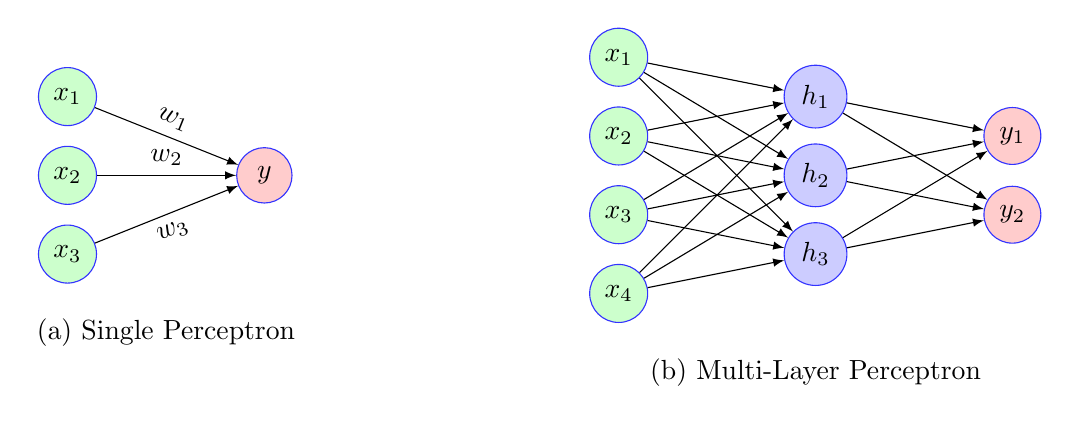
\begin{tikzpicture}[
    neuron/.style={circle, draw=blue!80, fill=blue!20, minimum size=20pt},
    input/.style={neuron, fill=green!20},
    output/.style={neuron, fill=red!20},
    >=latex
]
% Single Perceptron
\begin{scope}[xshift=-3cm]
    % Inputs
    \node[input] (x1) at (0,1) {$x_1$};
    \node[input] (x2) at (0,0) {$x_2$};
    \node[input] (x3) at (0,-1) {$x_3$};
    
    % Output neuron
    \node[output] (y) at (2.5,0) {$y$};
    
    % Connections
    \draw[->] (x1) -- node[above, sloped] {$w_1$} (y);
    \draw[->] (x2) -- node[above] {$w_2$} (y);
    \draw[->] (x3) -- node[below, sloped] {$w_3$} (y);
    
    % Title
    \node[align=center] at (1.25,-2) {(a) Single Perceptron};
\end{scope}

% Multi-Layer Perceptron
\begin{scope}[xshift=4cm]
    % Input layer
    \node[input] (i1) at (0,1.5) {$x_1$};
    \node[input] (i2) at (0,0.5) {$x_2$};
    \node[input] (i3) at (0,-0.5) {$x_3$};
    \node[input] (i4) at (0,-1.5) {$x_4$};
    
    % Hidden layer
    \node[neuron] (h1) at (2.5,1) {$h_1$};
    \node[neuron] (h2) at (2.5,0) {$h_2$};
    \node[neuron] (h3) at (2.5,-1) {$h_3$};
    
    % Output layer
    \node[output] (o1) at (5,0.5) {$y_1$};
    \node[output] (o2) at (5,-0.5) {$y_2$};
    
    % Connections for input to hidden layer
    \foreach \i in {1,2,3,4}
        \foreach \j in {1,2,3}
            \draw[->] (i\i) -- (h\j);
    
    % Connections for hidden to output layer
    \foreach \i in {1,2,3}
        \foreach \j in {1,2}
            \draw[->] (h\i) -- (o\j);
    
    % Title
    \node[align=center] at (2.5,-2.5) {(b) Multi-Layer Perceptron};
\end{scope}

\end{tikzpicture}
\caption{Neural Network Architectures\index{neural architectures}: (a) Single perceptron\index{perceptron!single} computing $y = \sigma(\sum_{i} w_i x_i + b)$\index{activation function}, where $\sigma$ is an activation function. 
(b) Multi-layer perceptron\index{perceptron!multi-layer} computing hidden layer\index{hidden layer} $h_j = \sigma(\sum_{i} w^{(1)}_{ij} x_i + b^{(1)}_j)$ followed by outputs\index{output layer} 
$y_k = \sigma(\sum_{j} w^{(2)}_{jk} h_j + b^{(2)}_k)$. This architecture enables learning complex non-linear mappings\index{non-linear mappings} through multiple layers of transformation\index{transformation layers}.}
\label{fig:neural_architectures}
\end{figure}

\noindent
Neural networks\index{neural networks!definition} have revolutionized modern machine learning\index{machine learning} by learning \emph{non-linear}\index{non-linear} mappings from input features\index{input features} to output predictions\index{output predictions} without the need for manually engineered features\index{feature engineering}. In the context of language modeling\index{language modeling}, neural networks are particularly powerful because they can encode and combine linguistic features\index{linguistic features} in high-dimensional spaces\index{high-dimensional spaces}, capturing nuances that simpler statistical models\index{statistical models} may overlook.

\subsection{Perceptrons and Multi-Layer Perceptrons (MLPs)}
\noindent
The \textbf{perceptron} (Figure~\ref{fig:neural_architectures}), introduced by Frank Rosenblatt in the late 1950s, is one of the earliest forms of a trainable neural network. It models a single neuron with:
\begin{enumerate}
    \item A set of input weights.
    \item A linear combination of inputs and weights.
    \item A non-linear activation function (e.g., step function).
\end{enumerate}
While a single perceptron can only represent linear decision boundaries, stacking multiple perceptrons in layers (known as a \textbf{Multi-Layer Perceptron}, or MLP) allows for the modeling of highly complex, non-linear relationships.

\begin{itemize}
    \item \textbf{Input Layer.} Receives the raw features, such as token embeddings in NLP.
    \item \textbf{Hidden Layers.} Non-linear transformations are applied in each layer. Common activation functions include $\text{ReLU}, \tanh, \text{sigmoid}$.
    \item \textbf{Output Layer.} Produces the final prediction, such as a probability distribution over the next token for language modeling.
\end{itemize}

\subsection{Forward and Backpropagation}\index{forward propagation}\index{backpropagation}
\noindent
Learning in neural networks typically involves two main steps:
\begin{itemize}
    \item \textbf{Forward Propagation.} The process of moving data through the network from input to output:
    
    \begin{itemize}
        \item \textbf{Input Layer Processing:}
            \begin{itemize}
                \item Raw input features enter the network
                \item Each feature is weighted according to learned parameters
                \item The weighted inputs are combined and passed through an activation function
            \end{itemize}
            
        \item \textbf{Hidden Layer Transformations:}
            \begin{itemize}
                \item Each hidden layer receives processed information from the previous layer
                \item The network learns increasingly complex representations at each layer
                \item Non-linear activation functions allow the network to model complex patterns
                \item Each neuron acts as a feature detector, learning to recognize specific patterns
            \end{itemize}
            
        \item \textbf{Output Layer Generation:}
            \begin{itemize}
                \item The final layer produces predictions based on all previous transformations
                \item Output format depends on the task (e.g., probabilities for classification)
                \item The network's prediction is compared to the true target to compute error
            \end{itemize}
            
        \item \textbf{Key Concepts:}
            \begin{itemize}
                \item Information flows in one direction: input → hidden layers → output
                \item Each connection has a weight that's learned during training
                \item Bias terms allow the network to shift activation functions
                \item The network builds a hierarchical representation of the input data
            \end{itemize}
    \end{itemize}
    
    \begin{equation}\label{eq:forward_prop}
        \mathbf{z}^{(l)} = \mathbf{W}^{(l)} \mathbf{h}^{(l-1)} + \mathbf{b}^{(l)}, \quad \mathbf{h}^{(l)} = \sigma(\mathbf{z}^{(l)})
    \end{equation}
    where $\sigma(\cdot)$ is a non-linear activation function\index{activation function}, and $\mathbf{h}^{(0)} \equiv \mathbf{x}$ is the input vector\index{input vector}.

    \item \textbf{Backward Propagation (Backprop).}\index{backpropagation!definition} The backbone of neural network training\index{training}, backpropagation enables neural networks to learn from their mistakes through:
    \begin{itemize}
        \item \textbf{Error Attribution:}
            \begin{itemize}
                \item Determines how much each neuron contributed to the network's error
                \item Traces the path of mistakes backwards through the network
                \item Identifies which weights need the most adjustment
                \item Helps understand which parts of the network are most responsible for incorrect predictions
            \end{itemize}
            
        \item \textbf{Learning Process:}
            \begin{itemize}
                \item Adjusts weights to minimize prediction errors
                \item Stronger corrections for neurons that contributed more to mistakes
                \item Weaker corrections for neurons that had less impact
                \item Balances the influence of different network components
            \end{itemize}
            
        \item \textbf{Optimization Benefits:}
            \begin{itemize}
                \item Efficiently updates millions of parameters simultaneously
                \item Prevents the need for trial-and-error weight adjustment
                \item Enables deep networks to learn complex patterns
                \item Provides a systematic way to improve network performance
            \end{itemize}
            
        \item \textbf{Training Insights:}
            \begin{itemize}
                \item Helps identify learning problems (e.g., vanishing gradients)
                \item Guides the choice of learning rates and optimization strategies
                \item Indicates which parts of the network are learning effectively
                \item Assists in debugging network architectures
            \end{itemize}
    \end{itemize}

    \begin{itemize}
        \item \textbf{Chain Rule Application:} For a composite function $f(g(x))$, the chain rule states:
        \begin{equation}
            \frac{\partial f(g(x))}{\partial x} = \frac{\partial f}{\partial g} \cdot \frac{\partial g}{\partial x}
        \end{equation}
        
        \item \textbf{Gradient Flow:}\index{gradient flow} Starting from the output layer\index{output layer} and moving backward:
        \begin{enumerate}
            \item Compute loss gradient\index{loss gradient}: $\frac{\partial \mathcal{L}}{\partial \hat{\mathbf{y}}}$
            \item For each layer $l$, compute:
                \begin{align}
                    \frac{\partial \mathcal{L}}{\partial \mathbf{z}^{(l)}} &= \frac{\partial \mathcal{L}}{\partial \mathbf{h}^{(l)}} \cdot \frac{\partial \mathbf{h}^{(l)}}{\partial \mathbf{z}^{(l)}} \\
                    \frac{\partial \mathcal{L}}{\partial \mathbf{W}^{(l)}} &= \frac{\partial \mathcal{L}}{\partial \mathbf{z}^{(l)}} \cdot \frac{\partial \mathbf{z}^{(l)}}{\partial \mathbf{W}^{(l)}}
                \end{align}
        \end{enumerate}
        
        \item \textbf{Parameter Updates:} Using computed gradients, parameters are updated:
        \begin{equation}
            \mathbf{W}^{(l)} \leftarrow \mathbf{W}^{(l)} - \alpha \frac{\partial \mathcal{L}}{\partial \mathbf{W}^{(l)}}
        \end{equation}
        where $\alpha$ is the learning rate.
    \end{itemize}

    Modern deep learning frameworks like PyTorch and TensorFlow implement automatic differentiation, computing these gradients efficiently without manual derivation. However, understanding the underlying mathematics remains crucial for:
    \begin{itemize}
        \item Debugging training issues
        \item Implementing custom layers
        \item Optimizing network architectures
        \item Choosing appropriate learning rates and optimization strategies
    \end{itemize}


    The learning rate $\alpha$ is a crucial hyperparameter that controls how large steps we take during training. A large learning rate means taking bigger steps, potentially learning faster but risking overshooting the optimal solution. A small learning rate takes smaller, more careful steps, leading to more stable training but requiring more time to converge. Finding the right learning rate is often a balancing act: too large and the training might diverge, too small and the training might be impractically slow or get stuck in local minima.
\end{itemize}


This loop of forward and backward propagation, repeated over multiple \emph{epochs} of training data, enables a neural network to \emph{learn} complex transformations—an essential capability for tasks like language modeling.

\noindent
An epoch represents one complete pass through the entire training dataset. During each epoch:
\begin{itemize}
    \item Every training example is used once for forward propagation
    \item The network's predictions are compared with true values
    \item Weights are updated through backpropagation
    \item The process is repeated for multiple epochs until the network converges
\end{itemize}

\noindent
Training typically requires multiple epochs because:
\begin{itemize}
    \item The network needs repeated exposure to learn complex patterns
    \item Initial weight updates may be suboptimal
    \item Different aspects of the data may be learned in different epochs
    \item The learning process is iterative and gradual
\end{itemize}

\subsection{Activation Functions}
\noindent
Activation functions impart non-linearity, allowing neural networks to model non-trivial functions. Without activation functions, neural networks would be limited to linear transformations, regardless of their depth. Here's why they're essential:

\begin{itemize}
    \item \textbf{Non-linearity:} Real-world problems rarely follow linear patterns. Activation functions enable networks to learn and represent complex, non-linear relationships in data.
    
    \item \textbf{Feature Transformation:} Each neuron can learn to activate for different input patterns, effectively becoming specialized feature detectors.
    
    \item \textbf{Gradient Flow:} Different activation functions affect how gradients flow through the network during training, influencing learning dynamics.
    
    \item \textbf{Output Range:} Activation functions can bound outputs to specific ranges (e.g., [0,1] for sigmoid, [-1,1] for tanh), which is useful for tasks like probability prediction.
\end{itemize}

See Figure \ref{fig:activation_functions} for a comparison of common activation functions.

\begin{figure}[h]
\centering
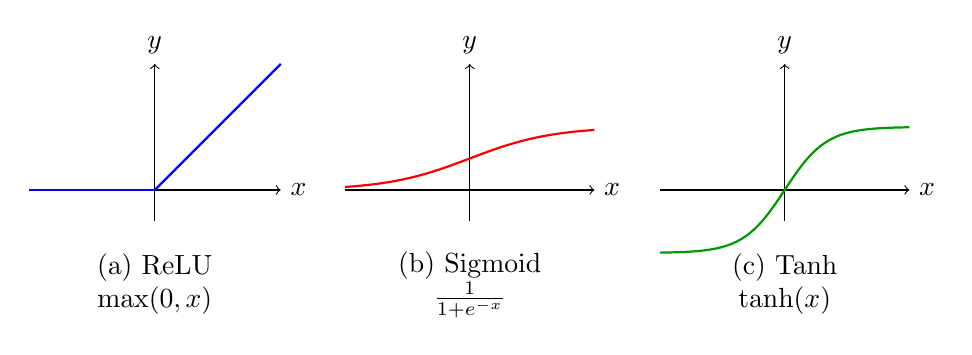
\begin{tikzpicture}[
    declare function={
        relu(\x) = max(0,\x);
        sigmoid(\x) = 1/(1 + exp(-\x));
        tanhy(\x) = (exp(\x) - exp(-\x))/(exp(\x) + exp(-\x));
    },
    scale=0.8
]
% Grid and axes for ReLU
\begin{scope}[xshift=-5cm]
    \draw[->] (-2,0) -- (2,0) node[right] {$x$};
    \draw[->] (0,-0.5) -- (0,2) node[above] {$y$};
    \draw[thick, blue] (-2,0) -- (0,0);
    \draw[thick, blue] (0,0) -- (2,2);
    \node[align=center] at (0,-1.5) {(a) ReLU\\$\max(0,x)$};
\end{scope}

% Grid and axes for Sigmoid
\begin{scope}[xshift=0cm, xscale=0.66]
    \draw[->] (-3,0) -- (3,0) node[right] {$x$};
    \draw[->] (0,-0.5) -- (0,2) node[above] {$y$};
    \draw[thick, red, domain=-3:3, samples=100] 
        plot (\x,{sigmoid(\x)});
    \node[align=center] at (0,-1.5) {(b) Sigmoid\\$\frac{1}{1+e^{-x}}$};
\end{scope}

% Grid and axes for Tanh
\begin{scope}[xshift=5cm, xscale=0.66]
    \draw[->] (-3,0) -- (3,0) node[right] {$x$};
    \draw[->] (0,-0.5) -- (0,2) node[above] {$y$};
    \draw[thick, green!60!black, domain=-3:3, samples=100] 
        plot (\x,{tanhy(\x)});
    \node[align=center] at (0,-1.5) {(c) Tanh\\$\tanh(x)$};
\end{scope}

\end{tikzpicture}
\caption{Common activation functions used in neural networks: (a) ReLU is simple and effective but suffers from the dying ReLU problem, (b) Sigmoid maps to $(0,1)$ but can saturate, (c) Tanh maps to $(-1,1)$ with stronger gradients near zero compared to sigmoid.}
\label{fig:activation_functions}
\end{figure}

\begin{itemize}
    \item \textbf{ReLU (Rectified Linear Unit):} 
    \begin{equation}\label{eq:relu}
        \sigma(z) = \max(0, z)
    \end{equation}
    Efficient and popular, though it can cause `dying ReLU' issues.
    
    \item \textbf{Sigmoid:}\index{sigmoid}\index{activation functions!sigmoid} 
    \begin{equation}\label{eq:sigmoid}
        \sigma(z) = \frac{1}{1+e^{-z}}
    \end{equation}
    Outputs values in $(0,1)$, but can saturate for large $|z|$.
    
    \item \textbf{Tanh:}\index{tanh}\index{activation functions!tanh} 
    \begin{equation}\label{eq:tanh}
        \sigma(z) = \tanh(z) = \frac{e^z - e^{-z}}{e^z + e^{-z}}
    \end{equation}
    A shifted and scaled version of the sigmoid function, outputs values in $(-1, 1)$. Also prone to saturation.
\end{itemize}

\subsection{Minimal Neural Network Example}
\noindent
The following code is a minimal example in Python of a single hidden-layer neural network for a binary classification task:

\begin{pythoncode}[Minimal Neural Network Example]
    import numpy as np
    import torch
    import torch.nn as nn
    from torch.utils.data import DataLoader
    
    # Part 1: Network Architecture and Initialization
    # ---------------------------------------------
    input_size = D
    hidden_size = H
    output_size = 1  # for binary classification
    
    # Initialize parameters
    W1 = np.random.normal(0, 0.01, (D, H))  # or torch.randn for PyTorch
    b1 = np.zeros(H)
    W2 = np.random.normal(0, 0.01, (H, output_size))
    b2 = np.zeros(output_size)
    
    
    # Part 2: Forward Pass Implementation
    # ---------------------------------
    def forward(x):
        # First layer
        z1 = x @ W1 + b1
        h1 = np.maximum(0, z1)  # ReLU activation
        
        # Output layer
        z2 = h1 @ W2 + b2
        y_pred = 1 / (1 + np.exp(-z2))  # sigmoid activation
        
        return y_pred, (z1, h1, z2)  # Return activations for backprop
    
    
    # Part 3: Backpropagation Implementation
    # ------------------------------------
    def compute_gradients(loss, y_pred, cache, x, y_true):
        z1, h1, z2 = cache
        
        # Gradient of loss with respect to output
        dy_pred = (y_pred - y_true) / len(y_true)
        
        # Gradients for output layer
        dz2 = dy_pred * y_pred * (1 - y_pred)  # sigmoid derivative
        dW2 = h1.T @ dz2
        db2 = np.sum(dz2, axis=0)
        
        # Gradients for hidden layer
        dh1 = dz2 @ W2.T
        dz1 = dh1 * (z1 > 0)  # ReLU derivative
        dW1 = x.T @ dz1
        db1 = np.sum(dz1, axis=0)
        
        return {'W1': dW1, 'b1': db1, 'W2': dW2, 'b2': db2}
    
    
    # Part 4: Training Loop
    # -------------------
    learning_rate = 0.01
    
    for epoch in range(num_epochs):
        for x_batch, y_batch in data_loader:
            # Forward pass
            y_pred, cache = forward(x_batch)
            
            # Compute binary cross-entropy loss
            loss = -np.mean(
                y_batch * np.log(y_pred) + 
                (1 - y_batch) * np.log(1 - y_pred)
            )
            
            # Compute gradients
            grads = compute_gradients(loss, y_pred, cache, x_batch, y_batch)
            
            # Update parameters
            W1 -= learning_rate * grads['W1']
            b1 -= learning_rate * grads['b1']
            W2 -= learning_rate * grads['W2']
            b2 -= learning_rate * grads['b2']
    \end{pythoncode}

\noindent
While this example is basic, the core ideas of forward propagation, loss computation, and backpropagation remain the same in more advanced architectures used in modern NLP tasks.

\subsection{Optimization Challenges}
\noindent
Despite their remarkable flexibility, neural networks are not without pitfalls. Common optimization challenges include:
\begin{itemize}
    \item \textbf{Vanishing/Exploding Gradients.} Deeper networks or RNNs may run into gradient magnitudes that become either too small or too large, slowing or destabilizing training.
    \item \textbf{Overfitting.} A network with many parameters can easily memorize the training data. Techniques such as \emph{dropout}, \emph{weight decay}, and \emph{batch normalization} help mitigate overfitting.
    \item \textbf{Choosing Hyperparameters.} Finding the right learning rate, batch size, and network architecture often involves empirical experimentation.
\end{itemize}

\noindent
Understanding these fundamental concepts is crucial before diving into more specialized architectures, such as Transformers. By grounding ourselves in the mechanics of standard neural networks, we lay the foundation for comprehending how modern LLMs leverage and extend these principles to handle vast amounts of textual data at massive scales.

\section{Overfitting and Regularization}\index{overfitting}\index{regularization}
\label{sec:overfitting_regularization}

\noindent
In the context of Large Language Models\index{LLM!overfitting}, overfitting occurs when a model performs well on training data\index{training data} but fails to generalize\index{generalization} to unseen examples. This section explores common regularization techniques\index{regularization techniques} used to combat overfitting in neural networks\index{neural networks!regularization}, with particular attention to their application in transformer-based architectures\index{transformer!regularization}.

\subsection{Understanding Overfitting}\index{overfitting!understanding}
\noindent
Overfitting manifests when a model learns to:
\begin{itemize}
    \item Memorize training examples\index{memorization} rather than learning generalizable patterns\index{patterns!generalizable}
    \item Capture noise\index{noise} in the training data rather than underlying relationships\index{relationships!underlying}
    \item Perform significantly better on training data than validation data\index{validation data}, showing a large generalization gap\index{generalization gap}
\end{itemize}

\subsection{Common Regularization Techniques}\index{regularization!techniques}

\subsubsection{Dropout}\index{dropout}
\noindent
Dropout\index{dropout!mechanism} randomly deactivates neurons during training with probability $p$, forcing the network to learn redundant representations\index{redundant representations}:

\begin{equation}
\mathbf{h}_\text{dropout} = \mathbf{m} \odot \mathbf{h}, \quad \mathbf{m}_i \sim \text{Bernoulli}(p)
\end{equation}

where $\odot$ represents element-wise multiplication\index{element-wise multiplication}, and $\mathbf{m}$ is the dropout mask\index{dropout!mask}.

Key benefits include:
\begin{itemize}
    \item Prevents co-adaptation\index{co-adaptation} of neurons
    \item Acts as implicit model ensemble\index{model ensemble}
    \item Reduces overfitting without increasing computational cost\index{computational cost}
\end{itemize}

\subsubsection{Weight Decay (L2 Regularization)}\index{weight decay}\index{L2 regularization}
\noindent
Weight decay\index{weight decay!mechanism} adds a penalty term to the loss function\index{loss function} based on the magnitude of weights:

\begin{equation}
\mathcal{L}_\text{total} = \mathcal{L}_\text{original} + \lambda \sum_{w \in \text{weights}} \|w\|^2
\end{equation}

where $\lambda$\index{regularization strength} controls the strength of regularization. This technique:
\begin{itemize}
    \item Encourages smaller weight values\index{weight values}
    \item Promotes smoother model behavior\index{model behavior}
    \item Helps prevent extreme parameter values\index{parameter values}
\end{itemize}

\subsubsection{Early Stopping}\index{early stopping}
\noindent
Early stopping\index{early stopping!mechanism} monitors validation performance\index{validation performance} and stops training when performance begins to degrade:
\begin{itemize}
    \item Tracks validation metrics\index{validation metrics} across epochs\index{epochs}
    \item Implements patience\index{early stopping!patience} to avoid stopping too early
    \item Saves best model checkpoint\index{model checkpoint} based on validation performance
\end{itemize}

\subsection{Transformer-Specific Regularization}\index{transformer!regularization}

\subsubsection{Attention Dropout}\index{attention dropout}
\noindent
In transformer architectures\index{transformer!architecture}, dropout is applied at multiple locations:
\begin{itemize}
    \item Attention weights dropout\index{attention!weights dropout}
    \item Hidden state dropout\index{hidden state dropout}
    \item Feed-forward layer dropout\index{feed-forward dropout}
\end{itemize}

\subsubsection{Layer Normalization}\index{layer normalization}
\noindent
Layer normalization\index{layer normalization!mechanism} helps stabilize training by normalizing activations\index{activation normalization}:

\begin{equation}
\text{LayerNorm}(x) = \gamma \odot \frac{x - \mu}{\sqrt{\sigma^2 + \epsilon}} + \beta
\end{equation}

where $\gamma$ and $\beta$ are learnable parameters\index{learnable parameters}, and $\epsilon$ is a small constant for numerical stability\index{numerical stability}.

\subsection{Practical Considerations}\index{practical considerations}

\noindent
When implementing regularization techniques\index{regularization!implementation}, consider:
\begin{itemize}
    \item \textbf{Hyperparameter Selection:}\index{hyperparameter selection}
    \begin{itemize}
        \item Dropout rate\index{dropout!rate} (typically 0.1-0.5)
        \item Weight decay coefficient\index{weight decay!coefficient}
        \item Early stopping patience\index{patience}
    \end{itemize}
    
    \item \textbf{Monitoring:}\index{monitoring}
    \begin{itemize}
        \item Training vs. validation curves\index{learning curves}
        \item Parameter magnitude distributions\index{parameter distributions}
        \item Gradient statistics\index{gradient statistics}
    \end{itemize}
    
    \item \textbf{Combination Effects:}\index{regularization!combinations}
    \begin{itemize}
        \item Different techniques may interact\index{technique interactions}
        \item Need to balance multiple regularization methods\index{regularization balance}
        \item Consider computational overhead\index{computational overhead}
    \end{itemize}
\end{itemize}

\noindent
Effective regularization\index{regularization!effective} is crucial for training robust language models\index{language models!robustness} that generalize well to unseen data\index{generalization!unseen data} while maintaining computational efficiency\index{computational efficiency}.


% \begin{itemize}
%     \item Perceptrons, MLPs, activation functions
%     \item Forward/backpropagation mechanics
%     \item Optimization challenges (vanishing/exploding gradients, overfitting)
% \end{itemize}

% PROMPT: Elaborate on how regularization techniques help in NLP
\section{Regularization and Generalization}
\begin{itemize}
    \item Dropout, weight decay
    \item Early stopping
    \item Data augmentation (in NLP context)
\end{itemize}


\part{Transformer Architecture and Attention}
% PROMPT: Introduce the concept of attention in a broader ML context

\chapter{The Attention Mechanism}
% PROMPT: Show step-by-step derivation of the dot-product attention formula
\section{Self-Attention Defined}
\begin{itemize}
    \item Query, key, value formulation
    \item Dot-product attention math
    \item Masked self-attention for sequence tasks
\end{itemize}

% PROMPT: Justify the scaling factor in scaled dot-product attention
\section{Scaled Dot-Product Attention}
\begin{itemize}
    \item Why scaling is important
    \item Softmax temperature
    \item Complexity analysis
\end{itemize}

% PROMPT: Provide a small example demonstrating multi-head attention outputs
\section{Multi-Head Attention}
\begin{itemize}
    \item Splitting and recombining embeddings
    \item Benefits of multiple attention heads
    \item Mathematical notation for multi-head attention
\end{itemize}


\chapter{Transformer Encoder-Decoder Structure}
% PROMPT: Compare sinusoidal to learned positional embeddings
\section{Positional Encodings}
\begin{itemize}
    \item Sinusoidal positional embeddings: the math behind them
    \item Alternative positional encoding methods
\end{itemize}

% PROMPT: Expand on the role of layer normalization
\section{Encoder Block}
\begin{itemize}
    \item Layer normalization and its role in stable training
    \item Residual connections: rationale and benefits
\end{itemize}

% PROMPT: Clarify the difference between encoder self-attention and decoder self-attention
\section{Decoder Block}
\begin{itemize}
    \item Masked multi-head attention
    \item Encoder-decoder cross-attention
    \item Combining outputs for language generation
\end{itemize}

% PROMPT: Collect all the main formulas for easy reference
\section{Mathematical Notation of the Transformer}
\begin{itemize}
    \item Putting it all together with formulas (layer norms, attention, feedforward)
\end{itemize}


\part{Training Large Language Models}
% PROMPT: Discuss large-scale data pipelines in brief

\chapter{Language Modeling and Pretraining Objectives}
% PROMPT: Differentiate cross-entropy loss from perplexity
\section{Statistical Language Modeling}
\begin{itemize}
    \item Maximum likelihood estimation (MLE) for next-token prediction
    \item Cross-entropy loss and perplexity
\end{itemize}

% PROMPT: Outline how partial masking affects training stability
\section{Masked Language Modeling (MLM)}
\begin{itemize}
    \item BERT-style masked token prediction
    \item The math behind partial conditioning
\end{itemize}

% PROMPT: Emphasize left-to-right modeling for generation tasks
\section{Causal Language Modeling (CLM)}
\begin{itemize}
    \item GPT-style left-to-right prediction
    \item Training objective and computational considerations
\end{itemize}

% PROMPT: Compare objectives like next sentence prediction and permutation LM
\section{Next Sentence Prediction, Permutation LM, and Other Objectives}
\begin{itemize}
    \item How objectives influence model’s learned representations
\end{itemize}


\chapter{Large-Scale Optimization Techniques}
% PROMPT: Explain how mini-batch size impacts convergence
\section{Stochastic Gradient Descent at Scale}
\begin{itemize}
    \item Mini-batch sizing and distributed training
    \item Memory considerations (gradient checkpoints, etc.)
\end{itemize}

% PROMPT: Compare Adam, AdamW, and LAMB in a tabular format
\section{Adaptive Optimizers}
\begin{itemize}
    \item Adam, AdamW, LAMB, and their update rules
    \item Convergence issues and practical tips
\end{itemize}

% PROMPT: Provide a short tutorial on implementing mixed-precision training
\section{Gradient Accumulation and Mixed Precision Training}
\begin{itemize}
    \item FP16 vs. FP32
    \item Trade-offs between speed and numerical stability
\end{itemize}

% PROMPT: Show an example of learning rate warm-up schedule
\section{Hyperparameter Tuning}
\begin{itemize}
    \item Learning rate schedules (warm-up, decay)
    \item Regularization in large-scale settings
\end{itemize}


\chapter{Scaling Laws and Model Behavior}
% PROMPT: Cite recent papers on scaling laws
\section{Scaling Relationships}
\begin{itemize}
    \item Empirical laws for model size vs. performance
    \item Data size requirements
    \item Diminishing returns and capacity
\end{itemize}

% PROMPT: Theorize why overparameterization can sometimes improve generalization
\section{Mathematical Intuition for Overparameterization}
\begin{itemize}
    \item Why bigger might be better (lottery ticket hypothesis, double descent)
    \item Inductive biases learned by LLMs
\end{itemize}

% PROMPT: Mention typical hardware setups for large-scale training
\section{Practical Constraints}
\begin{itemize}
    \item Hardware limitations (GPU/TPU memory, compute time)
    \item Budgeting for training
\end{itemize}


\part{Advanced Topics and Future Directions}
% PROMPT: Highlight cutting-edge research in LLMs

\chapter{Fine-Tuning and Prompt Engineering}
% PROMPT: Show a side-by-side comparison of full fine-tuning vs. LoRA
\section{Methods of Fine-Tuning}
\begin{itemize}
    \item Full fine-tuning vs. parameter-efficient techniques (LoRA, adapters)
    \item Continual learning and catastrophic forgetting
\end{itemize}

% PROMPT: Demonstrate a few-shot prompting scenario
\section{Prompt Engineering and In-Context Learning}
\begin{itemize}
    \item Few-shot and zero-shot prompting
    \item The math behind attention re-weighting due to prompts
\end{itemize}

% PROMPT: Recommend metrics for zero-shot vs. fine-tuned models
\section{Evaluation Metrics and Challenges}
\begin{itemize}
    \item BLEU, ROUGE, perplexity, and beyond
    \item Human vs. automated evaluations
\end{itemize}


\chapter{Emergent Abilities and Interpretability}
% PROMPT: Give examples of complex reasoning tasks LLMs can handle
\section{Emergent Behaviors}
\begin{itemize}
    \item “Chain-of-thought” reasoning and large model capabilities
    \item Breakdown of tasks that LLMs excel at vs. struggle with
\end{itemize}

% PROMPT: Provide a sample attention visualization
\section{Interpretability Tools}
\begin{itemize}
    \item Attention visualization, gradient-based explanation
    \item Attribution methods (Integrated Gradients, etc.)
\end{itemize}

% PROMPT: Discuss how to measure and mitigate bias in LLMs
\section{Safety, Bias, and Ethics}
\begin{itemize}
    \item Mathematical perspectives on bias measurement
    \item Calibration, uncertainty, and fairness metrics
\end{itemize}


\chapter{Efficient Serving and Deployment}
% PROMPT: Compare quantization methods (e.g., 8-bit, 4-bit)
\section{Model Distillation and Compression}
\begin{itemize}
    \item Teacher-student framework
    \item Quantization, pruning, and the math behind it
\end{itemize}

% PROMPT: Illustrate how to handle batching during inference
\section{Latency Considerations}
\begin{itemize}
    \item Transformer inference optimizations (kernel fusion, GPU acceleration)
    \item Batch vs. streaming inference
\end{itemize}

% PROMPT: Propose different deployment strategies for large-scale LLMs
\section{Serving Architectures}
\begin{itemize}
    \item Distributed serving strategies
    \item Memory sharing and caching for LLMs
\end{itemize}


\chapter{Future Directions in Large Language Models}
% PROMPT: Explore new avenues of research in multimodality
\section{Multimodal Extensions}
\begin{itemize}
    \item Visual language models, audio-text models
    \item Cross-modal attention math
\end{itemize}

% PROMPT: Show how RLHF is formulated as a policy optimization problem
\section{Integration with Reinforcement Learning}
\begin{itemize}
    \item RLHF (Reinforcement Learning from Human Feedback)
    \item Policy gradients in the context of language generation
\end{itemize}

% PROMPT: Point to unsolved theoretical questions about LLM scaling
\section{Open Research Questions}
\begin{itemize}
    \item Efficient scaling, interpretability, and unsolved challenges
    \item Potential theoretical breakthroughs
\end{itemize}


\part{Conclusion and Resources}
% PROMPT: Summarize the key takeaways of the book

\chapter{Conclusion and Next Steps}
% PROMPT: Recap the most important mathematical concepts in a concise manner
\section{Summary of Key Mathematical Concepts}
\begin{itemize}
    \item From linear algebra to advanced optimization
\end{itemize}

% PROMPT: Provide concrete tips on bridging theory and practice
\section{Bridging Theory and Practice}
\begin{itemize}
    \item Implementation tips, code libraries, and frameworks
\end{itemize}

% PROMPT: Suggest external resources for continued learning
\section{Recommended Resources}
\begin{itemize}
    \item Research papers, online courses, open-source repositories
\end{itemize}

% PROMPT: Conclude with a futuristic perspective on LLMs
\section{Looking Ahead}
\begin{itemize}
    \item The ongoing evolution of LLM capabilities
    \item Encouraging readers to contribute to the field
\end{itemize}


\appendix
% PROMPT: Include proofs of key mathematical results in detail
\chapter{Mathematical Proofs and Derivations}
\begin{itemize}
    \item Detailed proofs for key theorems (e.g., convergence of optimization algorithms)
    \item Concentration inequalities for large models
\end{itemize}

% PROMPT: Provide a quick reference for all the mathematical symbols used
\chapter{Notation Guide}
\begin{itemize}
    \item Symbols used throughout the book
\end{itemize}

% PROMPT: Define important terms used in the text
\chapter{Glossary of Terms}
\begin{itemize}
    \item Definitions of key terms in deep learning, NLP, and mathematics
\end{itemize}

\end{document}
